\documentclass{ltugproc}

\usepackage[hybrid]{markdown}
\newcommand\term[1]{\textit{#1}}
\newcommand\command[1]{\texttt{#1}}
\newcommand\packagename[1]{\texttt{#1.sty}}
\newcommand\option[1]{\texttt{-\/-#1}}
% \usepackage{microtype}
\newcommand\texfourht{\term{\TeX4ht}}

\author{Michal Hoftich}
\title{\texfourht: LaTeX to Web publishing}
\begin{document}
\maketitle

\section{Introduction}
\texfourht\ is a system for conversion of \TeX\ documents to various output
formats, most notably several variants of \HTML, or \term{OpenDocument
Format}, supported by word processors such as Microsof Word or LibreOffice
Writer. 



The conversion process is started by a package \packagename{tex4ht}. It loads special 
configuration files for packages supported by \texfourht. These configuration files may fix clashes between the configured package and \texfourht, but most notably the package commands
can be patched to insert special marks, so called hooks. These hooks
are then populated with tags in the selected output format. 


\begin{figure*}[htp]
  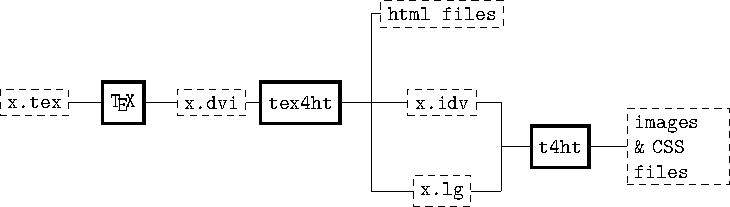
\includegraphics[width=\textwidth]{img/tex4ht_process.pdf}
\caption{\texfourht\ process overview}
\label{fig:overview}
\end{figure*}




\end{document}
